\subsection{Resultado - Exercício 3}

Os passos são:
\begin{itemize}[leftmargin=3.5em, itemsep=-.5mm, topsep=0.5mm]
    \item Transformar sin(x) em série.
    \item Aplicar a fórmula do resíduo e definir o tamanho da série
    \item Imprimir a função na forma de série e usando numpy no python
    \item Realizar os testes
    \item Apresentar o código Python e GnuPlot
 \end{itemize}

\subsubsection{Transformar $sin(x)$ em série.}
Temos os cálculos para escrever $sin(x)$ usando a Série de Taylor.
\begin{figure}[H]
    \centering
    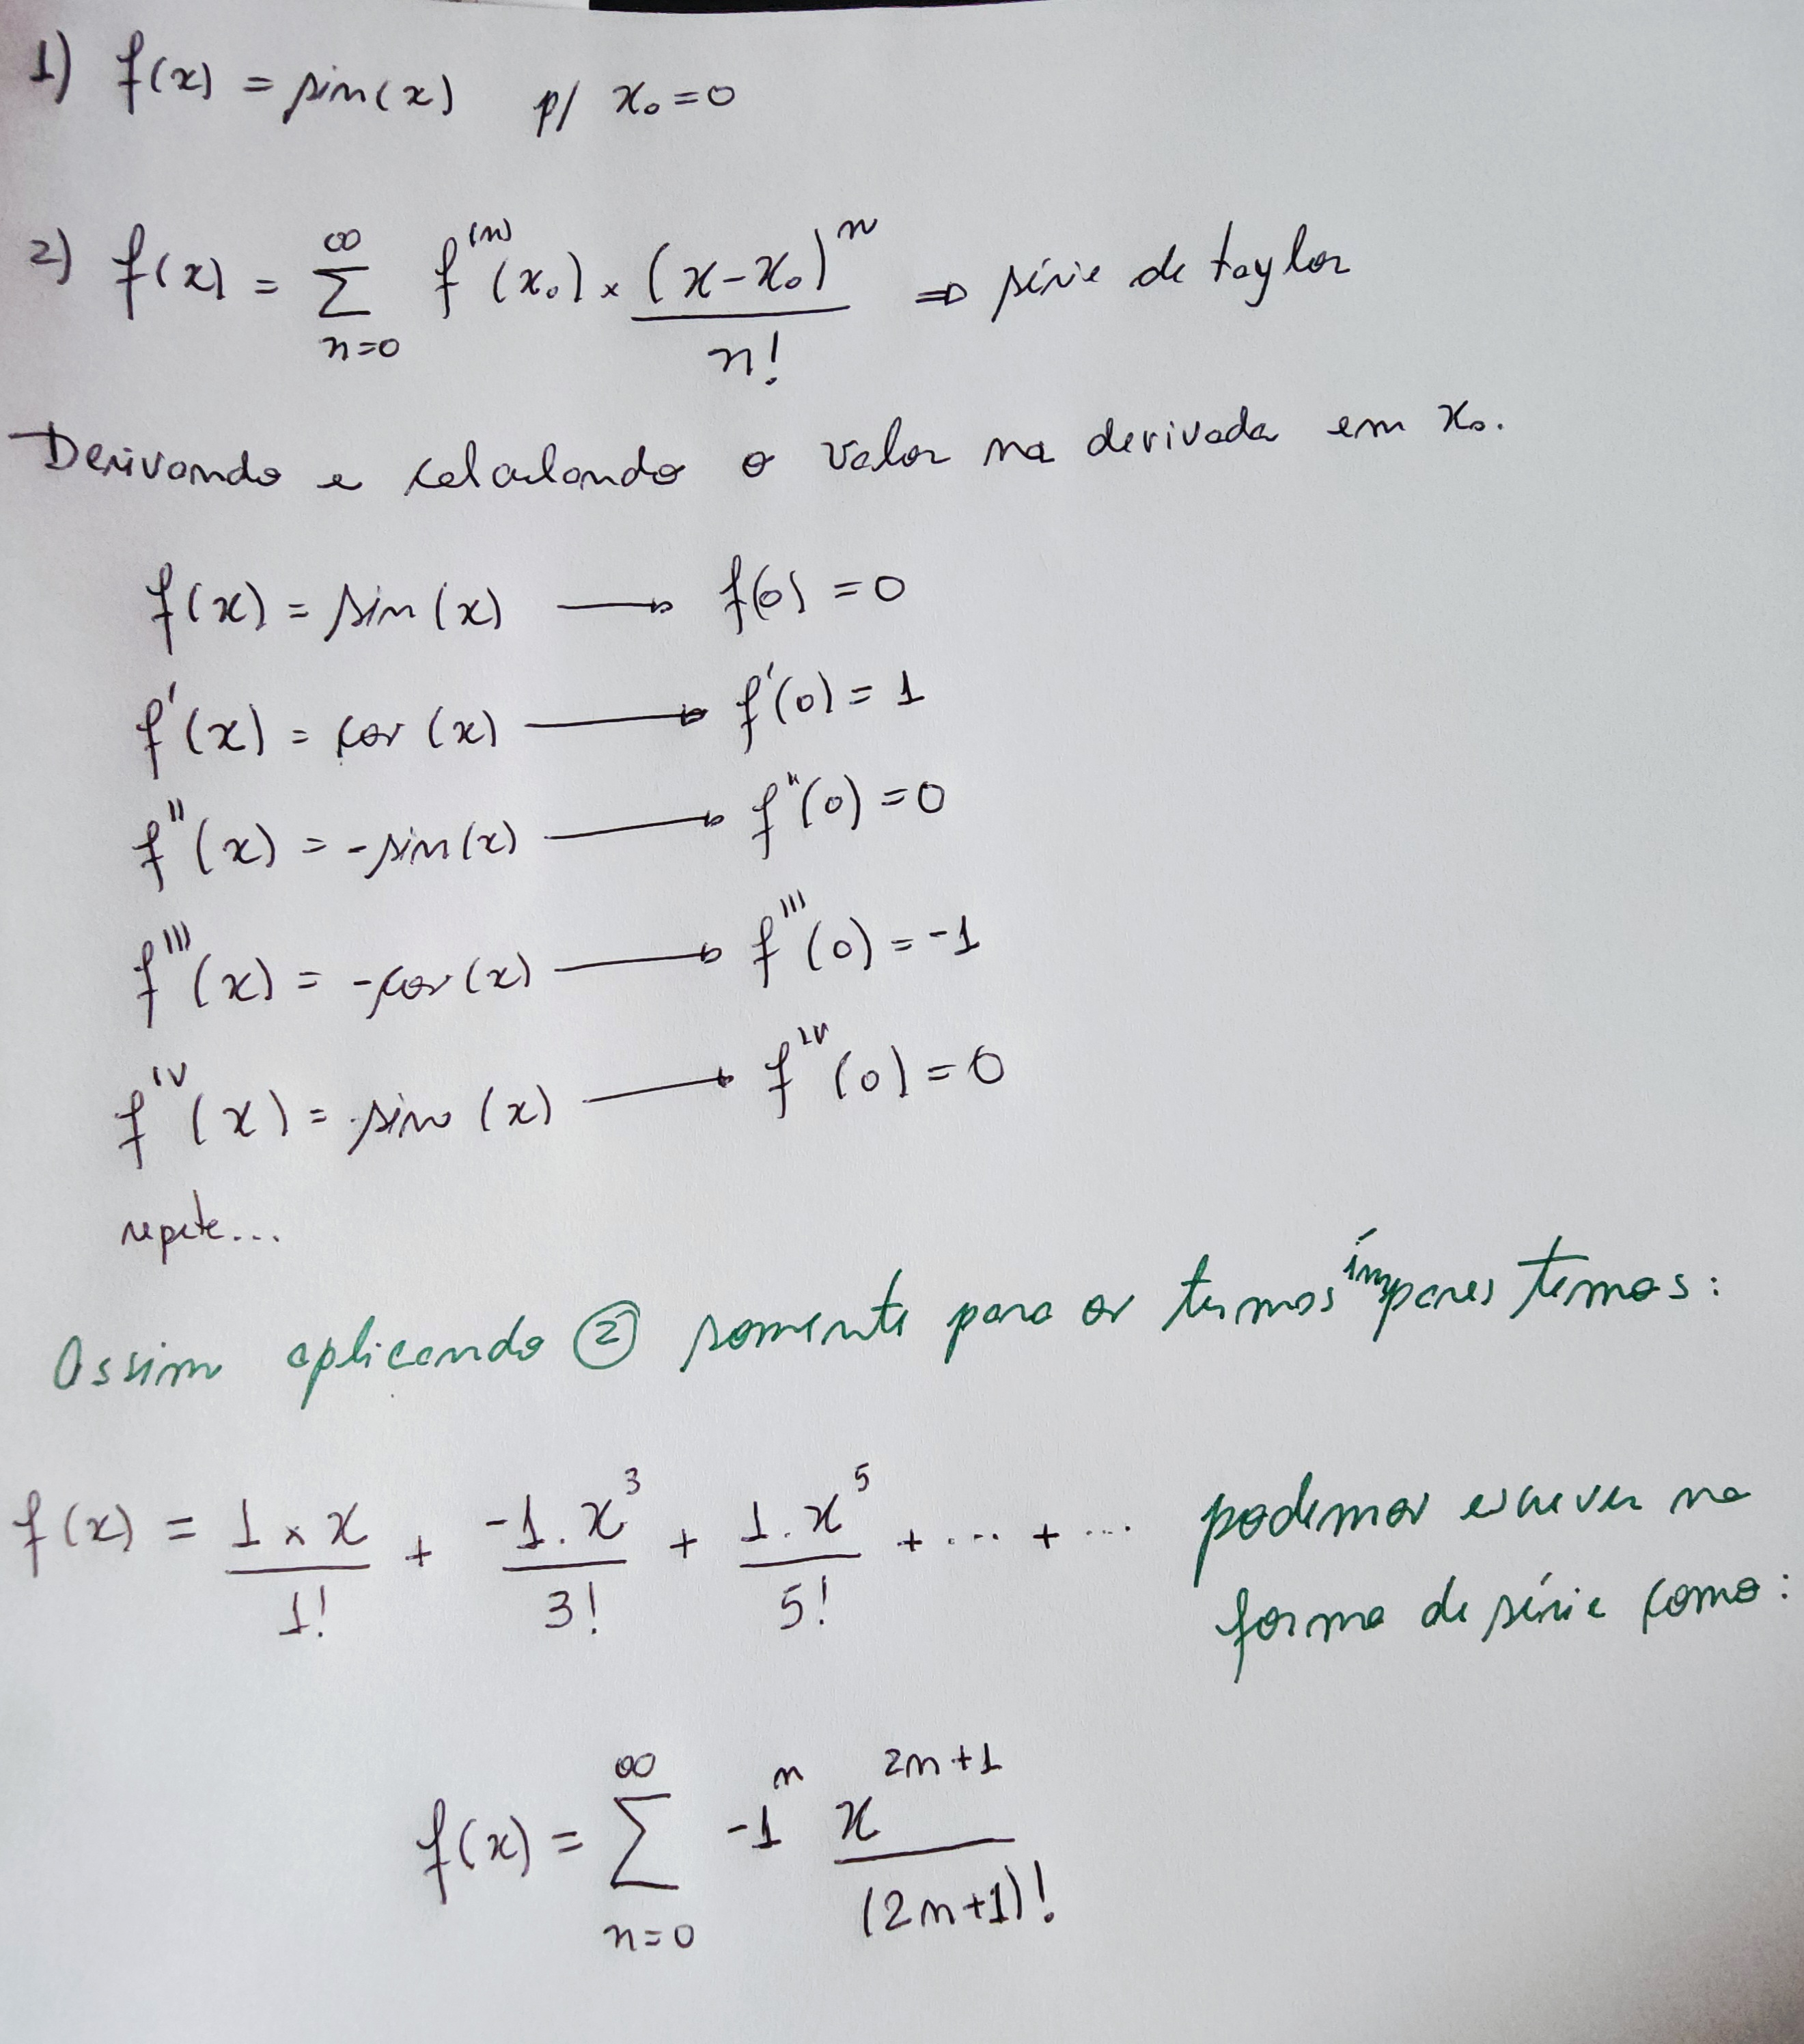
\includegraphics[width=.46\textwidth]{imagens/exercicio3_parte_1}
    \caption{Escrevendo $sin(x)$ na forma de série entre $0$ e $\frac{\pi}{2}$ obtemos como resultado $\sum_{n=0}^{\infty} -1^n \frac{x^{2 \cdot n + 1}}{(2 \cdot n + 1)!} $}
    \label{fig:lista_exercicio3_parte1}
\end{figure}
\newpage

\subsubsection{Aplicar a fórmula do resíduo e definir o tamanho da série}
Aplicando as Equações de resíduo de Taylor e o valor médio para integrais ponderadas temos:
\begin{figure}[H]
    \centering
    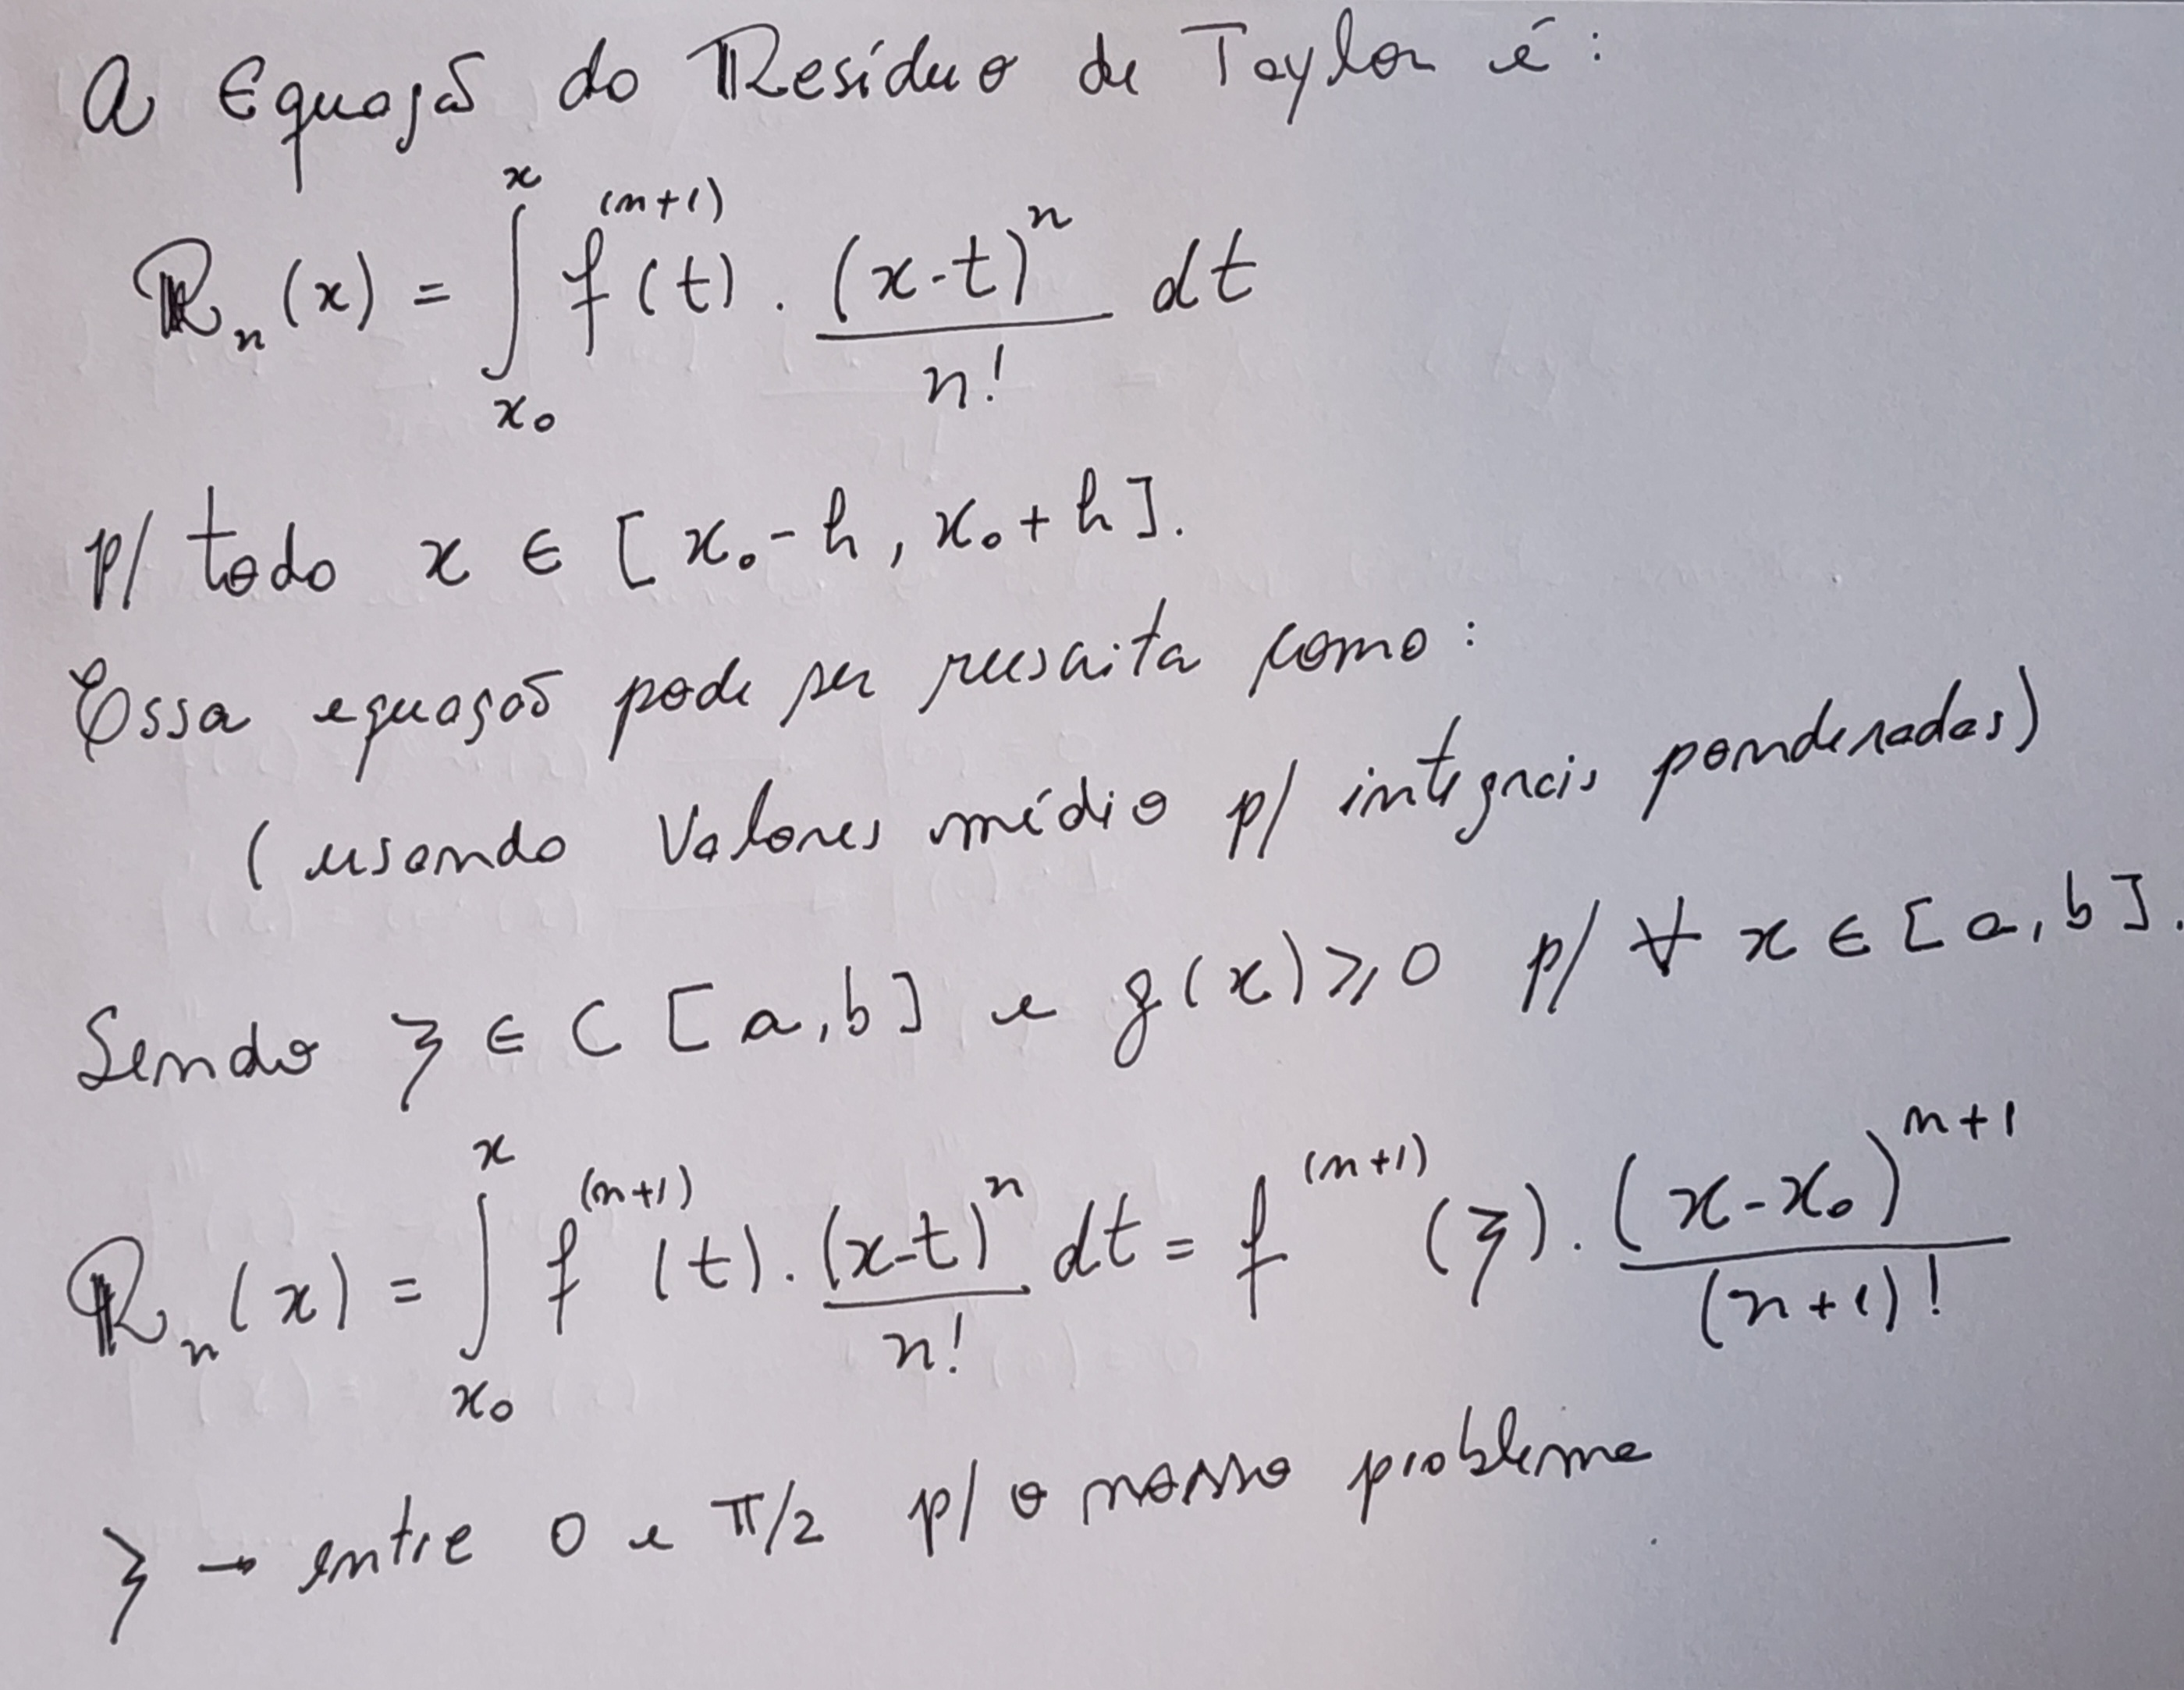
\includegraphics[width=.80\textwidth]{imagens/exercicio3_parte_2}
    \caption{Escrevendo o resíduo}
    \label{fig:lista_exercicio3_parte2}
\end{figure}
Continuando o raciocício e aplicando o resultado do resíduo.
\begin{figure}[H]
    \centering
    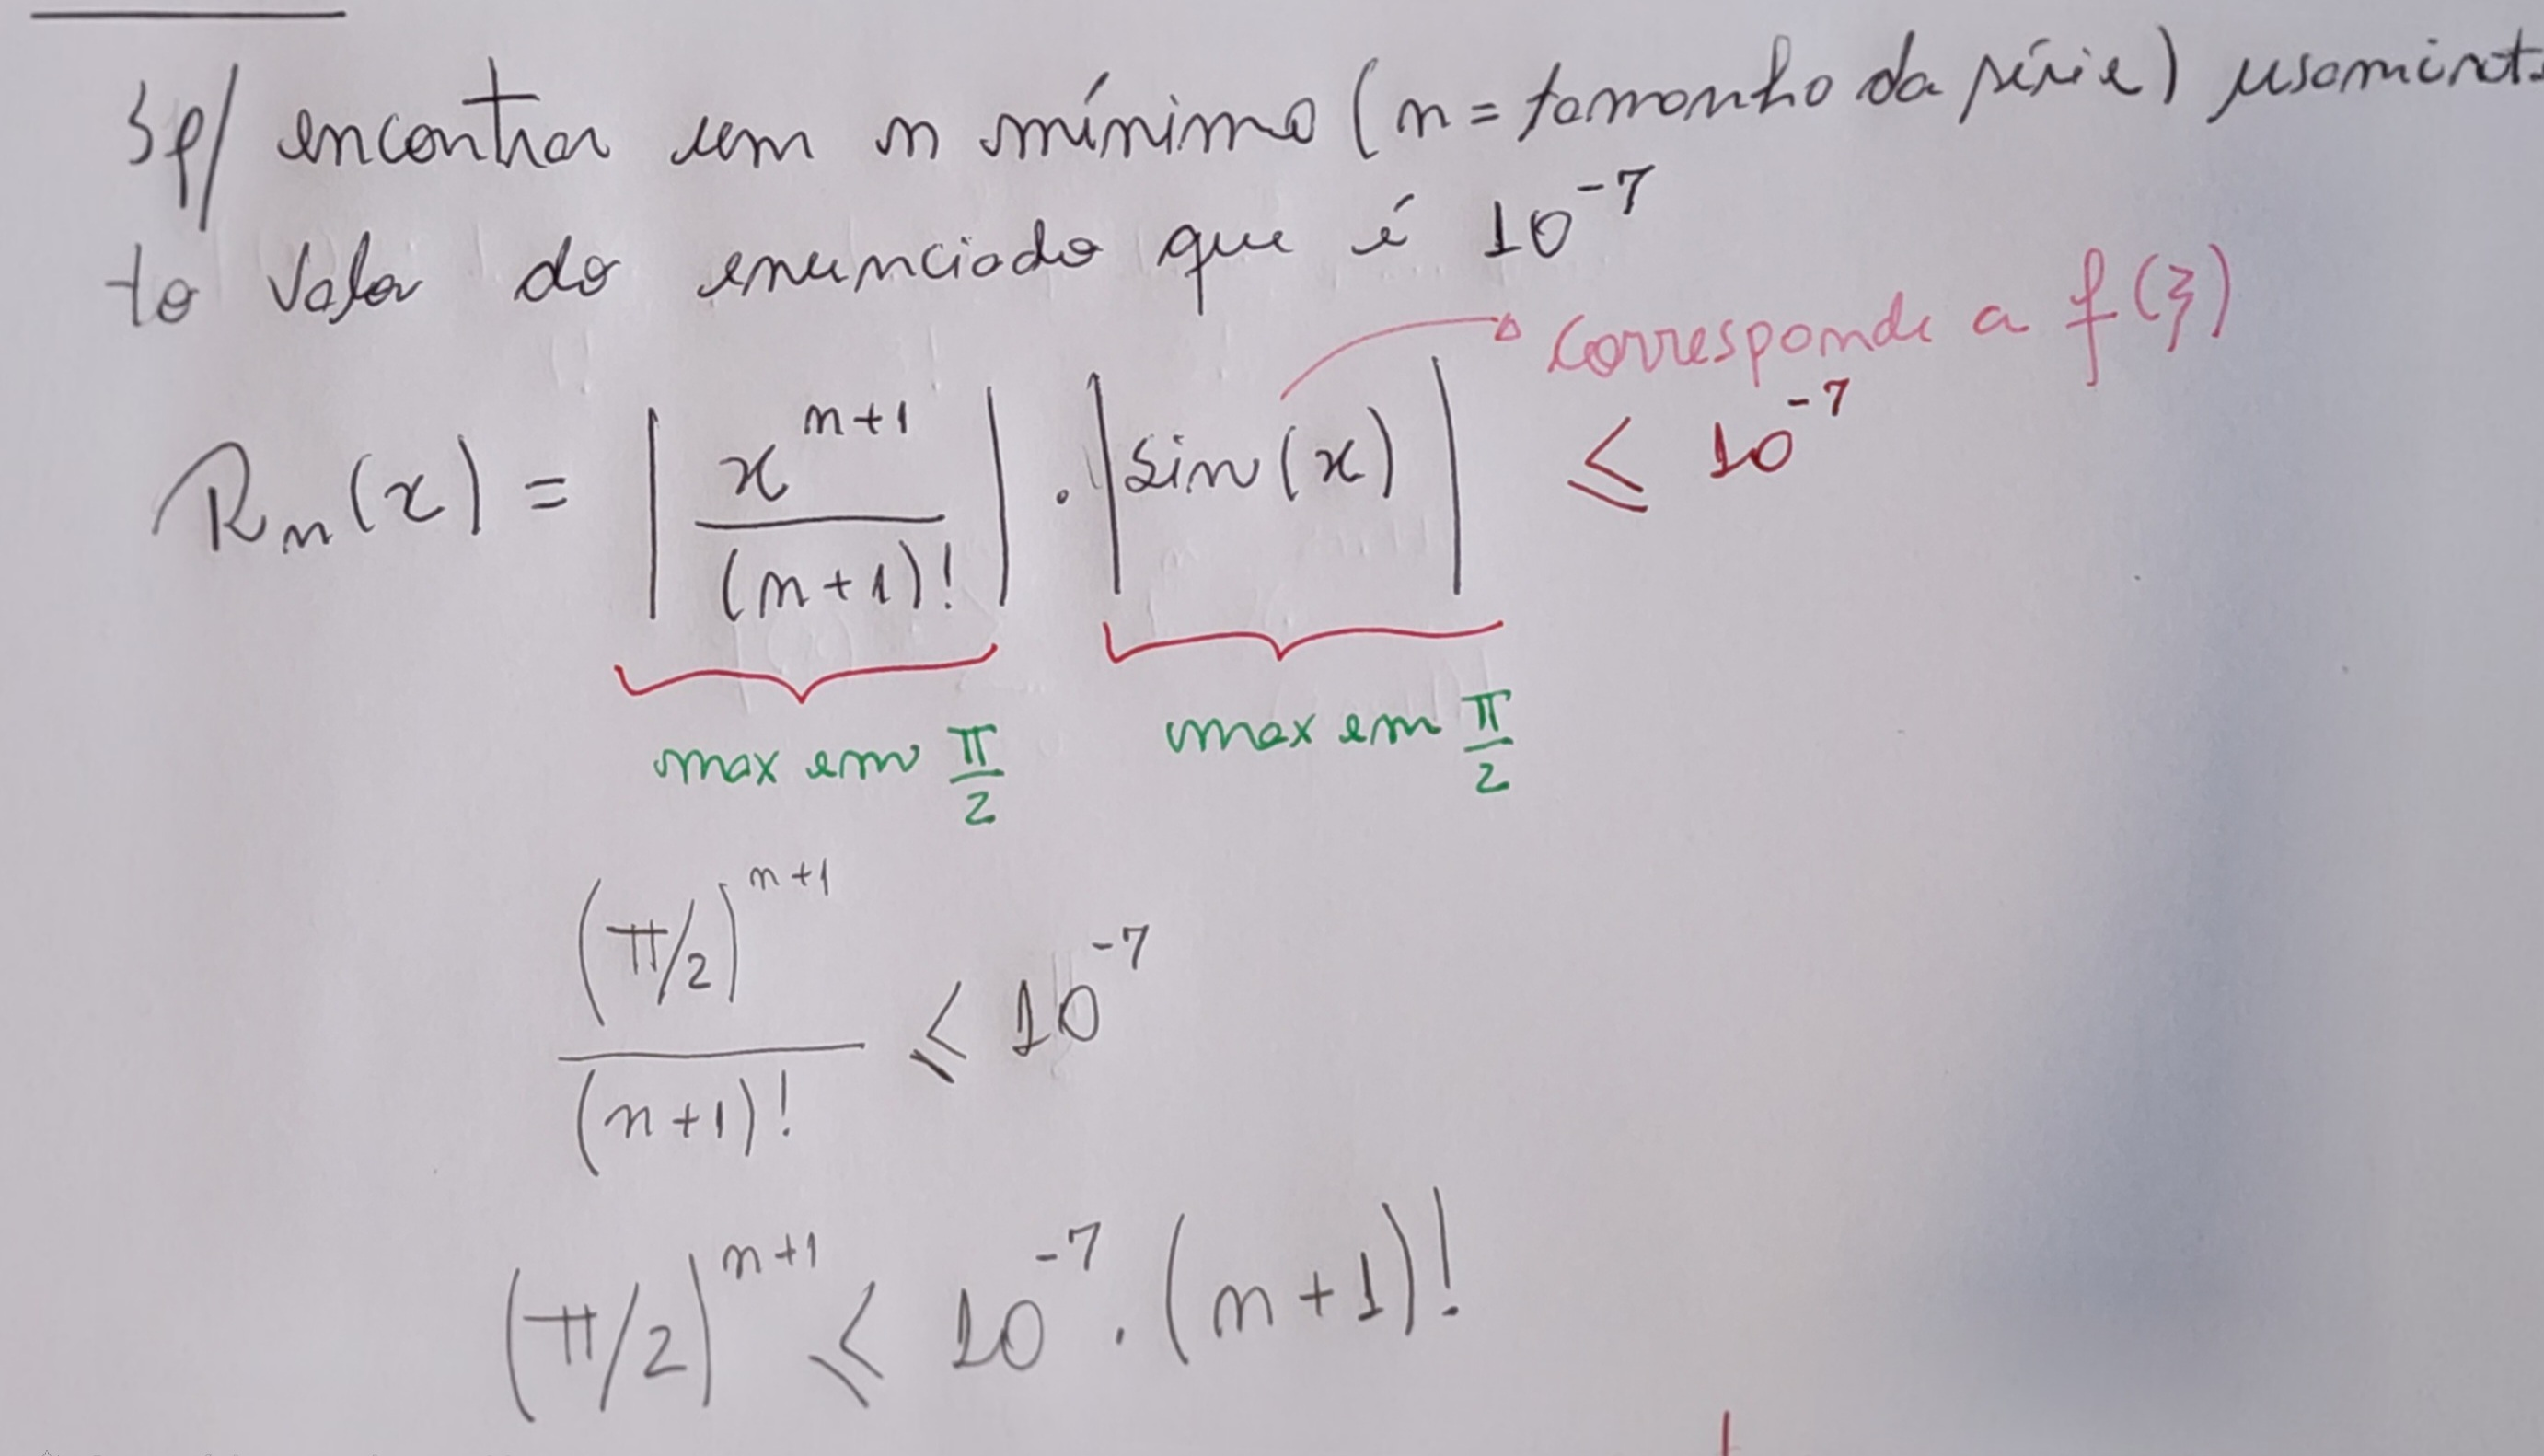
\includegraphics[width=.80\textwidth]{imagens/exercicio3_parte_3}
    \caption{Definindo a equação parar encontrar o valor de N. Essa equação foi testada com valores maiores que 2 e encontramos como verdadeiro o valor 13}
    \label{fig:lista_exercicio3_parte3}
\end{figure}

\input{tabela_residuos_exercicio3}

Usando a tabela Tabela~\ref{tab:exercicio_3_definir_grau_minimo} podemos ver que o menor grau que polinômio deve ter é 13. \\
Assim vamos definir 13 na chamada da função \texttt{calculaFTaylor} limitando o maior grau do polinômio em $\frac{x^{13}}{13!}$.

\subsubsection{Imprimir a função na forma de série e usando numpy no python}

Podemos ver nos gráficos da figura \ref{fig:grafico_exe3} que a diferença dos valores entre $-3 \cdot \pi$ a $3 \cdot \pi$ tem erros na ordem de $10^{-9}$ e que eles são maiores quando $ x = \frac{(2 \cdot n + 1)}{2} \cdot \pi $ para qualquer valor de n inteiro.
\begin{figure}[H]
    \centering
    \includegraphics[width=.95\textwidth]{imagens/exercicio3.png}
    \caption{Gráfico da função seno gerada por numpy e $P_2(x)$ e $P_{13}(x)$ e o módulo da diferença de $F(x)$ e $P_{13}(x)$}
    \label{fig:grafico_exe3}
\end{figure}


\subsubsection{Realizar os testes}


    \begin{table}[h!]
    \centering
    \caption{Testes do Exercicio 3}
    \begin{tabular}{|c|c|c|c|}
    \toprule
    \textbf{$x$} & \textbf{$f(x)$ (com NumPy)} & \textbf{$f(x)$ (com Taylor)} & \textbf{Diferenca} \\
    \midrule   
    7.0686e+00 & 7.0711e-01 & 7.0711e-01 & 1.1102e-16 \\
                            1.6493e+01 & -7.0711e-01 & -7.0711e-01 & 3.3307e-16 \\
                            3.2201e+01 & 7.0711e-01 & 7.0711e-01 & 6.6613e-16 \\
                            
    \bottomrule
    \end{tabular}
    \end{table}    
    

Vale lembrar que como temos valores muito próximos em uma subtração essa diferença pode ser um ruído de arredondamento.
Por outro lado, como o módulo da diferença é ordens de grandeza menor que o especificado ($10^{-7}$), esse erro satisfaz a necessidade da aplicação.\\

\subsubsection{Apresentar o código Python e GnuPlot}
\label{sec:caracteristicas-funcao-sin}
$sin(x)$ é função periódica e tem as simetrias de uma função impar. Assim ela foi limitanda com valores entre $0$ a $\frac{\pi}{2}$.
Isso está implementado na função \texttt{ajusta\_x\_calculo\_seno} usando as características de simetria e periodicidade do $sin(x)$.

\lstinputlisting[style=python]{scripts/exercicio3.py}
Código para a geração dos dados em Python.\\
\\
O Código em gnuplot lê o arquivo de dados e gera os gráficos usando um eixo x em múltiplos de PI para facilitar a leitura e com limites de range bem específicos para que fique o mais claro possível a sua leitura.\\
Além disso os 4 gráficos são agrupados em um único arquivo com alinhamento adequado para poder comparar os valores em x.
\lstinputlisting[style=gnuplot]{scripts/exercicio3.gnuplot}
Código em GnuPlot para geração dos gráficos do exercício3 baseado nos dados